\section{Introduction} \label{sec:introduction}

Recent advances in cellular automata have established rich frameworks for continuous-valued state spaces with flexible rule sets.
The Lenia project is particularly notable for the rich taxonomy of emergent behaviors that have been systematically and extensively characterized \citep{chan2020lenia,horibe2023exploring}.

Notable developments have also been made in incorporating differentiable frameworks to enable rule set development using gradient descent \citep{mordvintsev2020growing,hamon2022learning}.
Other approaches to discovering rule sets include evolutionary computation \citep{jain2024capturing}, quality-diversity search \citep{faldor2024toward}, and sampling from the representation space of LLMs (e.g., LLMs, computer vision, etc.) \citep{kumar2024automating}.
Rule sets may also be spatially localized within a cellular automata model and allowed to evolve in tandem with the state dynamics they enact within simulation \citep{plantec2023flowlenia}.

Pertinent references for cellular automata work within the realm of artificial life include,
\begin{enumerate}
\item Moveable Feast Machine \citep{ackley2023robust,ackley2019building,ackley2012movable},
\item Lenia \citep{chan2020lenia,chan2019lenia},
\item differentiable Lenia \citep{hamon2022learning},
\item particle Lenia \citep{mordvintsev2022particle},
\item flow Lenia \citep{plantec2023flowlenia},
\item neural cellular automata \citep{mordvintsev2020growing},
\item self-replicating neural cellular automata \citep{sinapayen2023selfreplication},
\item discretized differentiable cellular automata \citep{miotti2025differentiable}, and
\item earlier works include CAPOW \citep{griffeath2003new}, Larger than Life \citep{evans2001larger}, RealLife \citep{pivato2007reallife}, and SmoothLife \citep{rafler2011generalization}.
\end{enumerate}
In other areas of biological research, cellular automata approaches have also been applied in modeling physiological \citep{peak2004evidence,davidenko1992stationary}, ecological \citep{breckling2011cellular}, and social \citep{beltran2009forecasting} processes.

Although a major goal of work with cellular automata is as a platform to study eco-evolutionary processes, a key epistemological distinction of cellular automata approaches is that no explicit self-replicating unit is defined \citep{hamon2022learning}; instead, interest lies in the propagation of self-stabilizing ``soliton'' patterns in state space \citep{chan2019lenia}.
This enactivist approach contrasts agent-based, ``digital evolution'' approaches where an explicit self-replicating unit \citep{pennock2007models}.
Whereas such may be trivially tracked and characterized, implicit individuality introduces substantial challenges in tracking and characterizing eco-evolutionary dynamics within a simulation.

A key attractive aspect of cellular automata is in spatial locality of update rules, which makes evaluation well-suited to highly distributed processing \citep{ackley2023robust}.
Lenia, in particular, uses a local update rule based on element-wise convolution using fixed-size kernels.
Figure \ref{fig:lenia-pseudocode} provides pseudocode for the Lenia update function.
A nice visual overview of the Lenia update process can also be found at \url{https://developmentalsystems.org/sensorimotor-lenia/public/leniaVid.mp4}.

It is not hard to imagine how 2D or 3D lattice-based cellular automata with local update rules might effectively harness fabric-based hardware architectures such as the Cerebras Wafer-Scale Engine.
In fact, the Cerebras Software Development Kit (SDK) materials include an example implementation of Conway's Game of Life included with \citep{cerebras2024gol}.
Lenia, in particular, may potentially be compatible with an existing Field Equation modeling framework for the Wafer-Scale Engine \citep{woo2022disruptive}, which provides a higher-level, NumPy-like interface for programming on the Wafer-Scale Engine.
(Documentation for this project is hosted at \url{https://dirk-netl.github.io/WSE_FE/index.html}.)
Cerebras provides a PyTorch back-end, which may be helpful in working with neural Cellular Automata \citep{cerebras2022pytorch}.
Conveniently, reference code for differentiable Lenia used in prototype work for this project is implemented in PyTorch \citep{hamon2022learning}.

Past work with agent-based simulations on the Cerebras Wafer-Scale Engine have successfully applied hereditary stratigraphy methodology for decentralized phylogeny tracking \citep{moreno2024trackable}.
In brief, hereditary stratigraphy methodology works by attaching a small, fixed-size (e.g., 64 bit) heritable tag to agent genomes.
These tags undergo a specially-designed mutation process that allows fast, accurate estimation of the number of generations elapsed since the common ancestor of two tags.
As such, phylogenetic history within a simulation  (i.e., the ancestry tree among agents) can then be estimated from sample genomes, akin to how biologists build phylogenies by comparing similarities between organisms' DNA.

However, existing work leveraging the hereditary stratigraphy approach has assumed an explicit agent genome model and hooked into explicit agent replication events.
In this work, we explore how distributed phylogeny tracking via hereditary stratigraphy might be generalized to track interaction and/or replication dynamics in cellular automata-based simulations where explicit agent genomes and agent replication do not exist.

\subsection{Proposed Approach}

\begin{figure}
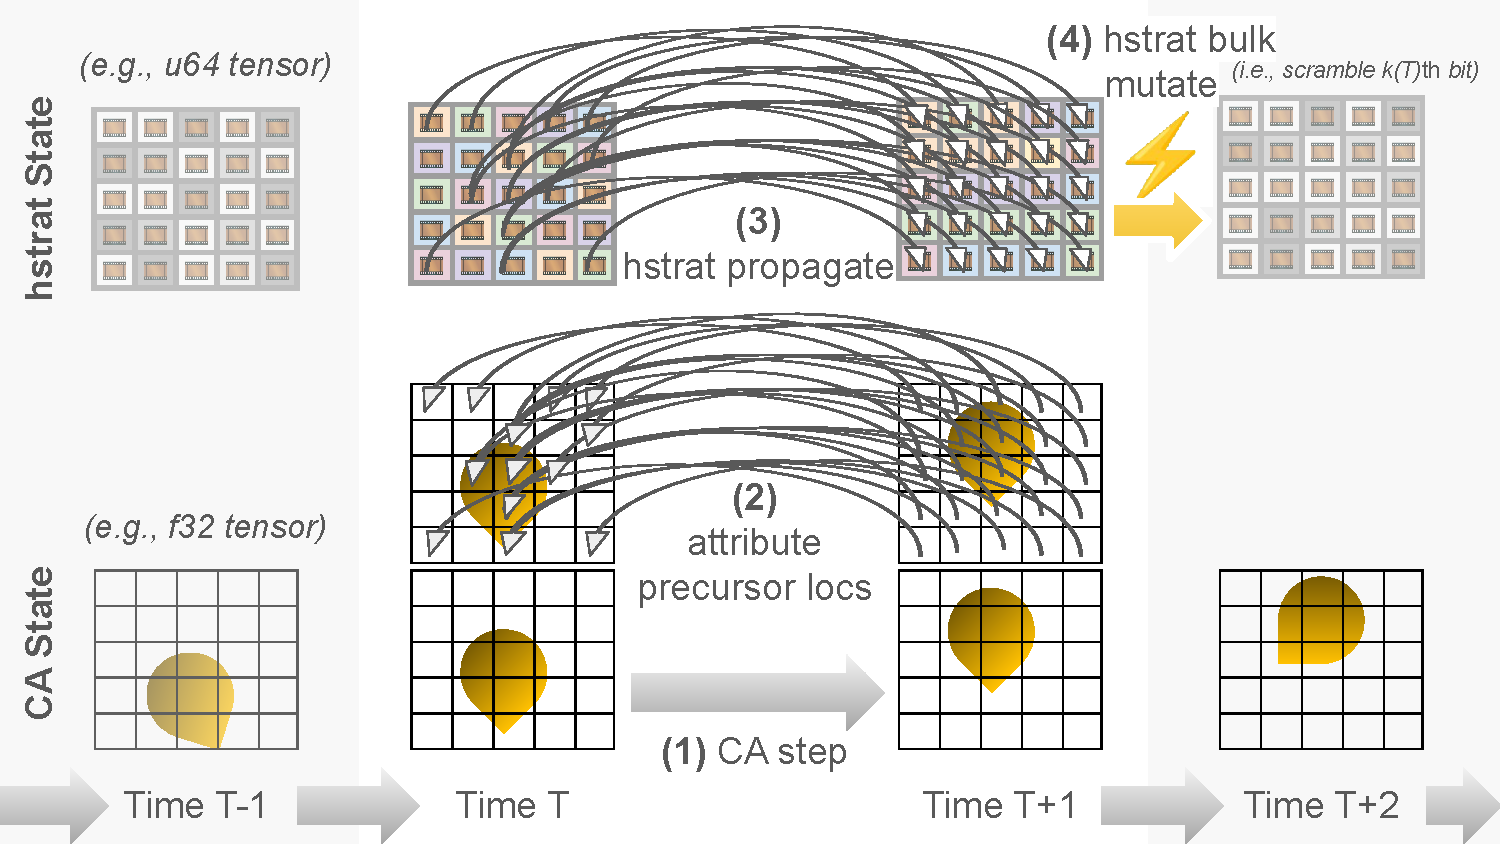
\includegraphics[width=0.8\textwidth]{img/hstrat-agentless-concept-schematic}
\caption{Proposed framework for incorporating distributed phylogeny tracking into CA systems.}
\label{fig:hstrat-agentless-concept}
\end{figure}


The proposed approach annotates each CA cell with dstream/hstrat annotation data.
(As per usual, dstream/hstrat annotations act as neutral instrumentation that do not influence simulation state.)
These annotations step forward synchronously with each CA update performed, meaning that semantic ``generations'' correspond to simulation timesteps.
Each update, dstream/hstrat annotations are ``propagated'' (copied) from current-timestep to next-timestep cells.
For this purpose, each timestep, an \textbf{attribution function} is calculated to generate a mapping from next-timestep cells within $A_{t+1}$ to current-timestep cells within $A_{t}$.
Next-timestep cells within $A_{t+1}$ then ``pull'' forward annotations from the current-timestep cell within $A_{t}$ they are attributed to.
For non-surjective attribution functions (i.e., where more than one next-timestep cell may be attributed to a single current-timestep cell), this propagation process naturally gives rise to a branching ``attribution tree'' structure.

Figure \ref{fig:hstrat-agentless-concept} provides a schematic overview of the proposed strategy for cellular automata phylogeny tracking.
Several desirable properties are worth noting,
\begin{itemize}
\item bulk updating many hstrat/dstream buffers synchronized to the same timestep is efficient (i.e., the $k(t)$'th bit of all items are randomized) and can be achieved through vectorized/matrix operations (e.g., NumPy, CuPy, JAX, etc.),
\item tracking data may be stored, managed, and transported directly through existing tensor/matrix frameworks (e.g., as u64 values),
\item tracking behavior can be configured in a modular/extensible manner by swapping attribution functions, and
\item in principle, it may be possible to design attribution functions robustly agnostic to unexpected/novel emergent soliton characteristics or behavior.
\end{itemize}
Additionally, existing desirable properties of hstrat/dstream-based tracking are preserved
\begin{itemize}
\item memory usage is fixed and known \textit{a priori},
\item tracking operations are fully decentralized,
\item tracking is robust to data loss, and
\item the methodology is well-suited to sampling-based data collection strategies.
\end{itemize}

Desirable properties of the attribution function and how such an attribution function should be formulated remain open questions.
One possible framing for tracking attribution trees that correspond to soliton phylogeny is to pursue a coalescent-like property: that attribution lineages for cells within the same soliton traced back in time should tend to rapidly converge to a "common ancestor."
It also may be desirable that attribution functions should avoid traces from one soliton back into another (i.e., to prevent ``contamination'' from non-reactive collisions between solitons).
In formulating an attribution function to track soliton phylogenies, it may be acceptable to act inertly over parts of a soliton's spatial footprint, so long as useful behavior occurs reliably within spatio-temporally coherent regions (e.g., regions of peak state density).

It is possible that ``flawed'' attribution trees that only approximately correspond to soliton phylogeny (or exhibit some other semantic tracking property entirely) may still generate useful information about cellular automata dynamics and/or history.
In this vein, more general applications for attribution trees could arise in tracking history within simulations modeling non-replicator/non-evolutionary systems.

The remainder of this section is organized into five further subsections, brainstorming possible project directions with respect to
\begin{enumerate}
\item capabilities to test,
\item ways to test,
\item configurations to test,
\item possible extensions, and
\item strategy limitations.
\end{enumerate}

Section \ref{sec:results} reports preliminary proof-of-concept work using a differentiable Lenia configuration exhibiting gliding solitons capable of autocatalytic self-replication \citep{hamon2022learning}.
This preliminary work applies a naive local-maximum attribution function with a manually-chosen radius.

\subsection{Capabilities to Test}

Questions about the properties/capabilities of the proposed methodology include,
\begin{enumerate}
\item tracking accuracy/behavior under discrete example scenarios of possible soliton interactions (Figure \ref{fig:lenia-event-types}),
\item accuracy versus ``ground truth'' phylogenies over the course of an entire simulation,
\item detecting and differentiating dynamics over the course of an entire simulation (e.g., presence/absence of solitons, soliton replication rate, the existence of distinct soliton configurations, types of soliton-soliton interaction, extrinsically-imposed spatial obstacles/state-purging/ruleset change, etc.),
\item performance/scalability (WSE? GPU via Jax?), and
\item generalizability across CA/Lenia flavors and parameter regimes.
\end{enumerate}

\subsection{Ways to Test}

Possible approaches to testing the proposed methodology include,
\begin{enumerate}
\item curate and manually label sample ``scenario episodes'' for case studies/benchmarking (e.g., Figure \ref{fig:lenia-event-types}),
\item compare attribution trees against ground-truth phylogeny extracted via computer vision tracker or manual annotation,
\item create attribution trees for mock/synthetic Lenia state sequences generated using a ``turtle''-like generator with explicit agents that may be tracked directly,
\item investigate whether CA parameter regimes are meaningfully reflected in the structure of extracted attribution trees.
\end{enumerate}

\begin{figure}
\centering
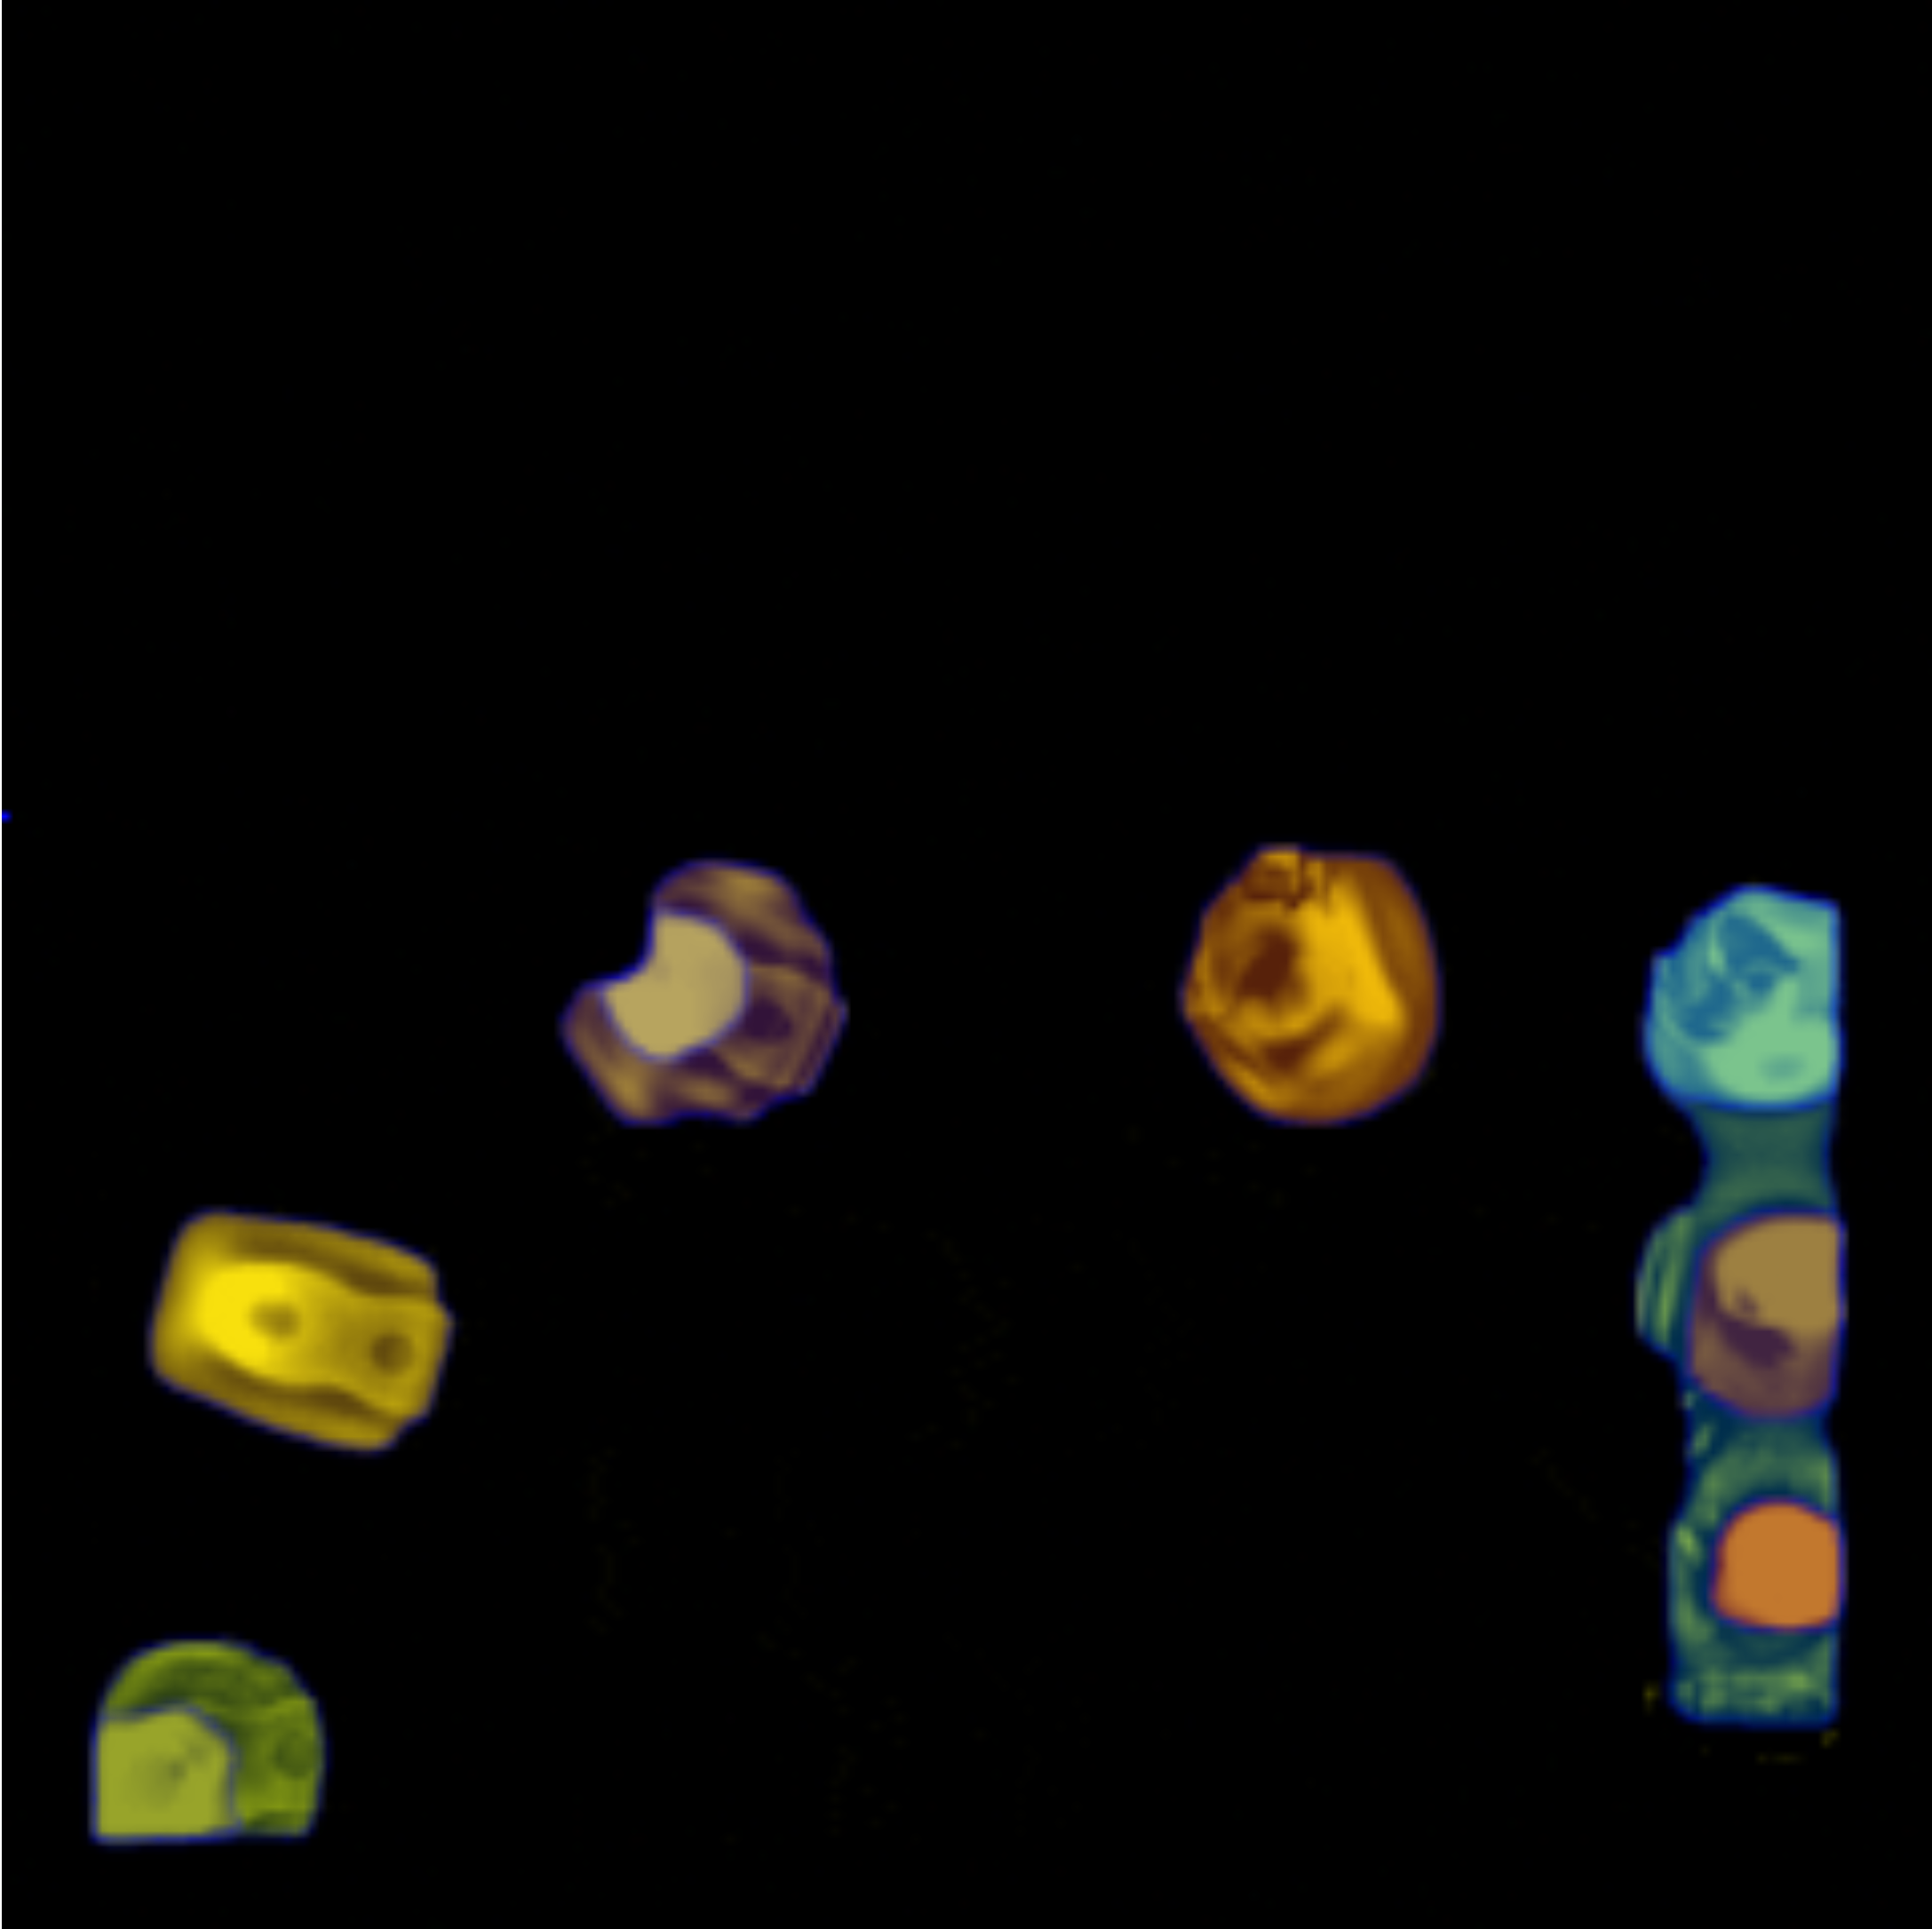
\includegraphics[width=0.5\textwidth]{img/sample-segment-anything}
\caption{Sample segmentation from segment anything \citep{kirillov2023segment}.}
\label{fig:sample-segment-anything}
\end{figure}


Recent developments in image segmentation tools (e.g., Meta's ``Segment Anything'') could make the computer vision tracking approach straightforward \citep{kirillov2023segment}.
However, a cursory search did not turn up completely no-fuss packaged off-the-shelf software for this purpose \citep{cheng2023segment,yang2023track}.
Figure \ref{fig:sample-segment-anything} shows an example result from feeding a Lenia frame through Segment Anything's online demo.

\subsection{Configurations to Test}

Experiments might be replicated across more than one CA system.
Within a CA system, experiments might compare rule sets producing different solitons and/or degraded/randomly generated rule sets that do not produce solitons.

With respect to available Lenia flavors, pre-existing example code that produces self-replicator solitons is available for differentiable \citep{hamon2022learning}, extended (``aquarium'') Lenia \citep{chan2020lenia}.
Three rule sets producing solitons, of which one appears to be a replicator, are provided with differentiable Lenia.
Notably, this project includes reproducible code for a deep-learning workflow to ``learn'' further rule sets exhibiting solitons \citep{hamon2022learning}.
Extended Lenia includes reproducible code with manually designed parameter sets for producing a replicator soliton and a non-replicator soliton \citep{chan2020lenia}.
An example replicator under base Lenia has also been described, although availability of reproducible code and parameter sets is uncertain \citep{chan2019lenia}.

Different attribution functions might also be compared.
Possible ingredients for formulating these attribution functions include,
\begin{itemize}
\item update-to-update state deltas,
\item derivative of a cell at time $t$ with respect to cell(s) at time $t-1$ (via differentiable update rules),
\item local maxima (current naive approach),
\item particles in Particle Lenia,
\item mass in Flow Lenia (attribution corresponding to propagation of local rule sets would be particularly interesting; however, robust replicators do not seem to be demonstrated in this framework),
\item trained/learned attribution based on labeled data, and
\item use of general-purpose, pre-trained foundation models (although these would need to be substantially stripped down to be practical).
\end{itemize}

\subsection{Extensions}

One possible methodological extension would be maintaining more than one independent tracking layer.
To get distinct behavior from these tracking layers, it would be necessary to use different attribution functions for each layer or add noise to the attribution function.
The latter noise-based strategy could be useful in detecting pairwise automatization or detecting the presence/extent of attribution ambiguity.

Attribution functions could be supplemented with ``clean-up'' processes that compare local annotation sets to purge rare/distantly related ``contamination'' attributions from solitons.

A common practice for Lenia projects is providing an accompanying Google Colab notebook reproducing major results.
Reusable/generalized software library tools might be developed for this purpose.

\subsection{Limitations}

Possible challenges and limitations of the proposed methodology include,
\begin{itemize}
\item achieving convergence within a soliton,
\item introduction of incomplete lineage sorting effects,
\item contamination of attribution trees by non-reactive soliton-soliton interactions,
\item difficulty meaningfully generalizing attribution functions across CA systems/flavors (particularly to CA with discrete state spaces \citep{miotti2025differentiable}).
\end{itemize}

This project direction may also be constrained by limited capabilities of existing cellular automata systems to generate rich/non-trivial eco-evolutionary dynamics.
